\begin{refsection}[research/maruyama/group.bib]
\nocite{*}
\chapter{HPC Programming Framework Research Team}

\section{Members}

\begin{itemize}
  \item[] Naoya Maruyama (Team Leader)
  \item[] Motohiko Matsuda (Research Scientist)
  \item[] Shinichiro Takizawa (Research Scientist)
  \item[] Mohamed Wahib (Postdoctoral Researcher)
  \item[] Keisuke Fukuda (Research Associate)
  \item[] Koji Ueno (Student Trainee)
  \item[] An Huynh (Student Trainee)
  \item[] Satoshi Matsuoka (Senior Visiting Scientist)
  \item[] Tomoko Nakashima (Assistant)
  \item[] Aya Motohashi (Assistant)
\end{itemize}

\section{Research Activities}

We develop high performance, highly productive software stacks that aim to simplify development of highly optimized, fault-tolerant computational science applications on current and future supercomputers, notably the K computer. Our current focus of work includes large-scale data processing, heterogeneous computing, and fault tolerance. A major ongoing project in our group will deliver a MapReduce runtime that is highly optimized for the intra- and inter-node architectures of the K computer as well as its peta-scale hierarchical storage systems. Another major project focuses on performance and productivity in large-scale heterogeneous systems. We also study high performance graph analytics on the K computer. Below is a brief summary of each project.

\section{Research Results and Achievements}

\subsection{KMR}
% Takizawa & Matsuda
\subsubsection{Improvng Locality When Running MPI Programs as MapReduce Tasks}

Although MapReduce systems can allocate tasks to nodes where their inputs reside to increase data locality for improving performance, these systems only target on tasks implemented as serial programs and do not consider running tasks implemented as parallel programs using MPI as Map or Reduce task.
As many scientific applications are implemented using MPI and some application workflows form ensemble execution patterns of such MPI programs, the workflows can be implemented easily and efficient data access can be achieved if a MapReduce system can allocate tasks implemented using MPI so that it can exploit data locality in them.

We proposed an extension of the execution model of MapReduce to achieve high performance when running MPI programs as Map/Reduce tasks.%~\cite{takizawa_hpc151}.
We model data to be processed as Key-Value as the traditional MapReduce model.
However, to processing the data, we propose a new \verb|map| function which makes process groups where each process in a group has a key-value whose key is same as those of other processes in the group and applies a user-defined mapper, which is implemented using MPI, to the key-values using processes in each group.
Figure~\localref{fig:kmr-01} shows the execution flow.

\begin{figure}
\centering
  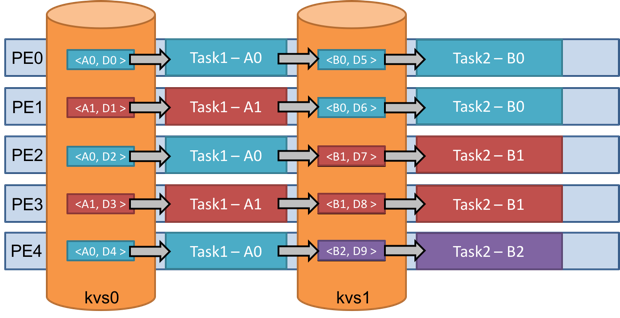
\includegraphics[width=0.5\textwidth,keepaspectratio,natwidth=193,natheight=40]
  {research/maruyama/lo01.png}
  \caption{Execution frow of MPI programm in MapReduce model}
  \locallabel{fig:kmr-01}
\end{figure}

To evaluate our proposal, we used $N \times N$ nodes of the K computer and compared performance of our method in which data access was performed locally and that of random data access.
We used a synthetic benchmark program where each node has an individual data and which iterates the following two computation; the first computation groups $N$ nodes in low direction and processes data on them, and the second groups $N$ nodes in column direction and processes data on them as showen in Figure~\localref{fig:kmr-02}.
The result is shown in Figure~\localref{fig:kmr-03}.
The horizontal axis is the amount of data on each node and the vertical axis is the relative performance of an iteration against random data access.
As can be seen from the figure, the performance of our proposal improve as the number of nodes and the amount of data increase.

\begin{figure}
\centering
  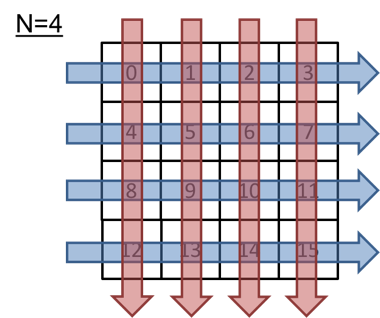
\includegraphics[width=0.5\textwidth,keepaspectratio,natwidth=193,natheight=40]
  {research/maruyama/lo02.png}
  \caption{Calculation pattern of the benchmark program}
  \locallabel{fig:kmr-02}
\end{figure}

\begin{figure}
\centering
  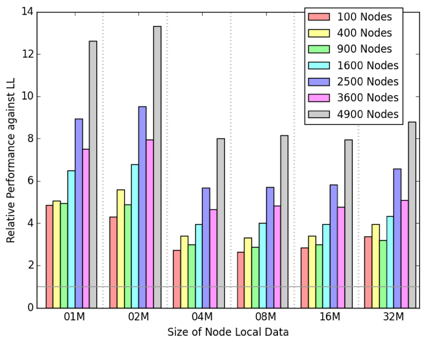
\includegraphics[width=0.5\textwidth,keepaspectratio,natwidth=193,natheight=40]
  {research/maruyama/lo03.png}
  \caption{Experimental results}
  \locallabel{fig:kmr-03}
\end{figure}


\subsubsection{Skew-Tolerant Shuffling for Load Balancing for Reduce Operation}

In a MapReduce program, the number of tasks in Map phase is defined by the number of split of the input data and that in Reduce phase is defined by the number of keys generated by the previous Map phase, and these numbers defines the maximum degree of parallelism of both phases.
Though the former can be defined by users when executing the program, users can not control the latter because it depends on patterns of applications and input data.
In contrast, as KMR statically defines number of processes used in both phase as the same value, we need to adopt load balancing techniques to average loads between processes in both phase.
Though balancing loads in Map phase can be left to users, a MapReduce system should support load balancing in Reduce phase as loads on processes heavily depend on the shuffle communication which is transparently performed by a system.

To balance loads on processes in Reduce phase, we proposed and implemented a shuffle algorithm that minimizes the skew of numbers of key-value pairs processed on each process~\cite{nishinaga_aics16}.
Our method is based an existing algorithm called LEEN and is extended as follows:
\begin{itemize}
\item It uses a distributed algorithm.
\item It reduces the number of search target keys (keys in key-value pairs) to reduce the cost of running the algorithm.
\end{itemize}
We compared the performance of our method and that of using a shuffle that randomly assigned key-values to processes by using a benchmark program that implemented k-means on top of MapReduce.
As a result, time spent for executing Reduce task was reduced against the random shuffle as our proposal averaged the number of keys among processes.
On the other hand, we also confirmed that the overall execution time increased due to the large cost of running the algorithm.
We plan to reduce the algorithm execution cost as a future work.

\subsubsection{Visualize MapReduce Task Execution}

Widely used MapReduce systems, such as Apache Hadoop and Spark, have their own profiling and visualization tools to see the status of jobs.
They help users to look for performance bottlenecks, to do debug and to optimize their programs.
As KMR is implemented as one of an MPI library using the C language, we can use any profilers, such as gprof, Intel Vtune and FUJITSU profiler.
However, as they target on low level events, such as memory access and function calls, they are not suitable for profiling task level events in a MapReduce program.
We developed an event tracer for KMR that traced MapReduce operations, such as Map/Reduce tasks and Shuffle communication, and a visualization tool named KMRViz that displayed the traces in a GUI window.

The tracer traces KMR function calls and records times of start and end of a function and numbers of input and output key-value pairs of the function.
To eliminate IO overhead for writing records during a program execution, we implemented the tracer so that it recorded profiles in-memory while execution and wrote them to files at the end of the program execution.
Moreover, to eliminate the burden of using the tracer, we implemented it so that the tracer could be enabled just by setting an environment variable.
KMRViz receives trace files generated by the tracer and displays them in time series by each process as the Figure~\localref{fig:kmrviz}.
It is implemented using GTK+3 and users can zoom-in and out using mice and trackpads.

\begin{figure}
\centering
  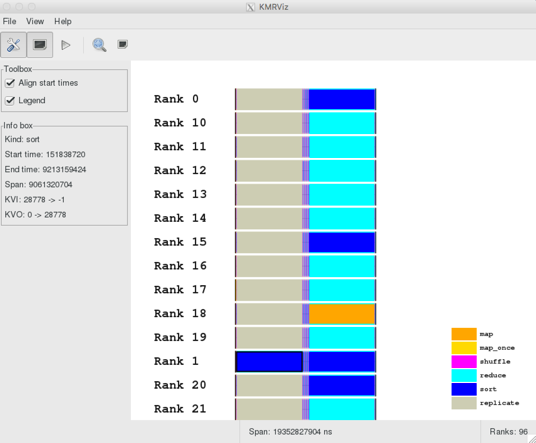
\includegraphics[width=0.5\textwidth,keepaspectratio,natwidth=193,natheight=40]
  {research/maruyama/kmrviz.png}
  \caption{Screenshot of KMRViz}
  \locallabel{fig:kmrviz}
\end{figure}


\subsection{High Level Framework for High Performance AMR}
% Wahib

\textbf{Summary:}
Adaptive Mesh Refinement methods reduce computational requirements of problems by increasing resolution for only areas of interest. However, in practice, efficient AMR implementations are difficult considering that the mesh hierarchy management must be optimized for the underlying hardware. Architecture complexity of GPUs can render efficient AMR to be particularity challenging in GPU-accelerated supercomputers. In this project, we present a high-level framework that can automatically transform serial uniform mesh code annotated by the user into parallel adaptive mesh code optimized for GPU-accelerated clusters. We show experimental results on three production applications. The speedups of code generated by our framework are comparable to hand-written AMR code while achieving good and weak scaling up to 1000 GPUs.

\textbf{Motivation:}
Frameworks that provide support for GPU in AMR applications require the programmer to write his own versions of the target-optimized solvers. Moreover, there can be scalability limitations caused by the overhead of the CPU-GPU communication schemes in those frameworks. We present a high-level framework that specializes in enabling efficient and scalable structured AMR solutions to scientific applications running on GPU-accelerated systems~\cite{Wahib2015}. Our framework uses a high-level programming model that provides an architecture-neutral programming interface and adopts an AMR strategy that would eliminate any CPU-GPU communication schemes that can limit scalability. We base our framework on octree-based AMR implementation in which we use a distributed tree and adapt the mesh in a parallel fashion with minimum inter-node communication. We base our GPU implementation on a data-centric approach at which the CPU is specialized in managing the data structures representing the mesh hierarchy, while AMR-specific routines that operate on mesh application data are executed on the GPU. Hence keeping the mesh application data arrays on the GPU memory for the entirety of the simulation.

\textbf{Programming model:}
The programming model is designed to be exposed in an architecture-neutral manner; the programmer has no knowledge of the underlying architecture. We provide the programmer with a set of C language directives to identify the stencil functions and data arrays in a logically fixed and uniform mesh implementation of solver(s). The programming interface enables the underlying compiler-based framework to statically analyze the solvers, construct the adaptive mesh hierarchy, automatically parallelize the mesh partition over distributed memory, and apply optimizations required for keeping the mesh application data, i.e., stencil arrays, in GPU memory throughout the simulation.

\textbf{Optimizations:}
When an AMR code generated by our framework is executed on a GPU-accelerated cluster, the stencil and mesh adaptation kernels run on the GPU, while managing the octree data structures and load balancing is done on the CPU side. Since we pursue efficiency and scalability, code on both the CPU and GPU should be optimized. The stencil kernel and mesh adaptation kernels are memory-bound kernels that are optimized to use the shared memory of the GPU and maintain coalesced memory accesses. For load balancing, \emph{intra-node} load balancing is applied by moving balancing the number of blocks equally among the GPUs. For the \emph{inter-node} load balancing, we rely on a space fitting curve to decide on how to redistribute the blocks.
\begin{figure*}[t]
\centering
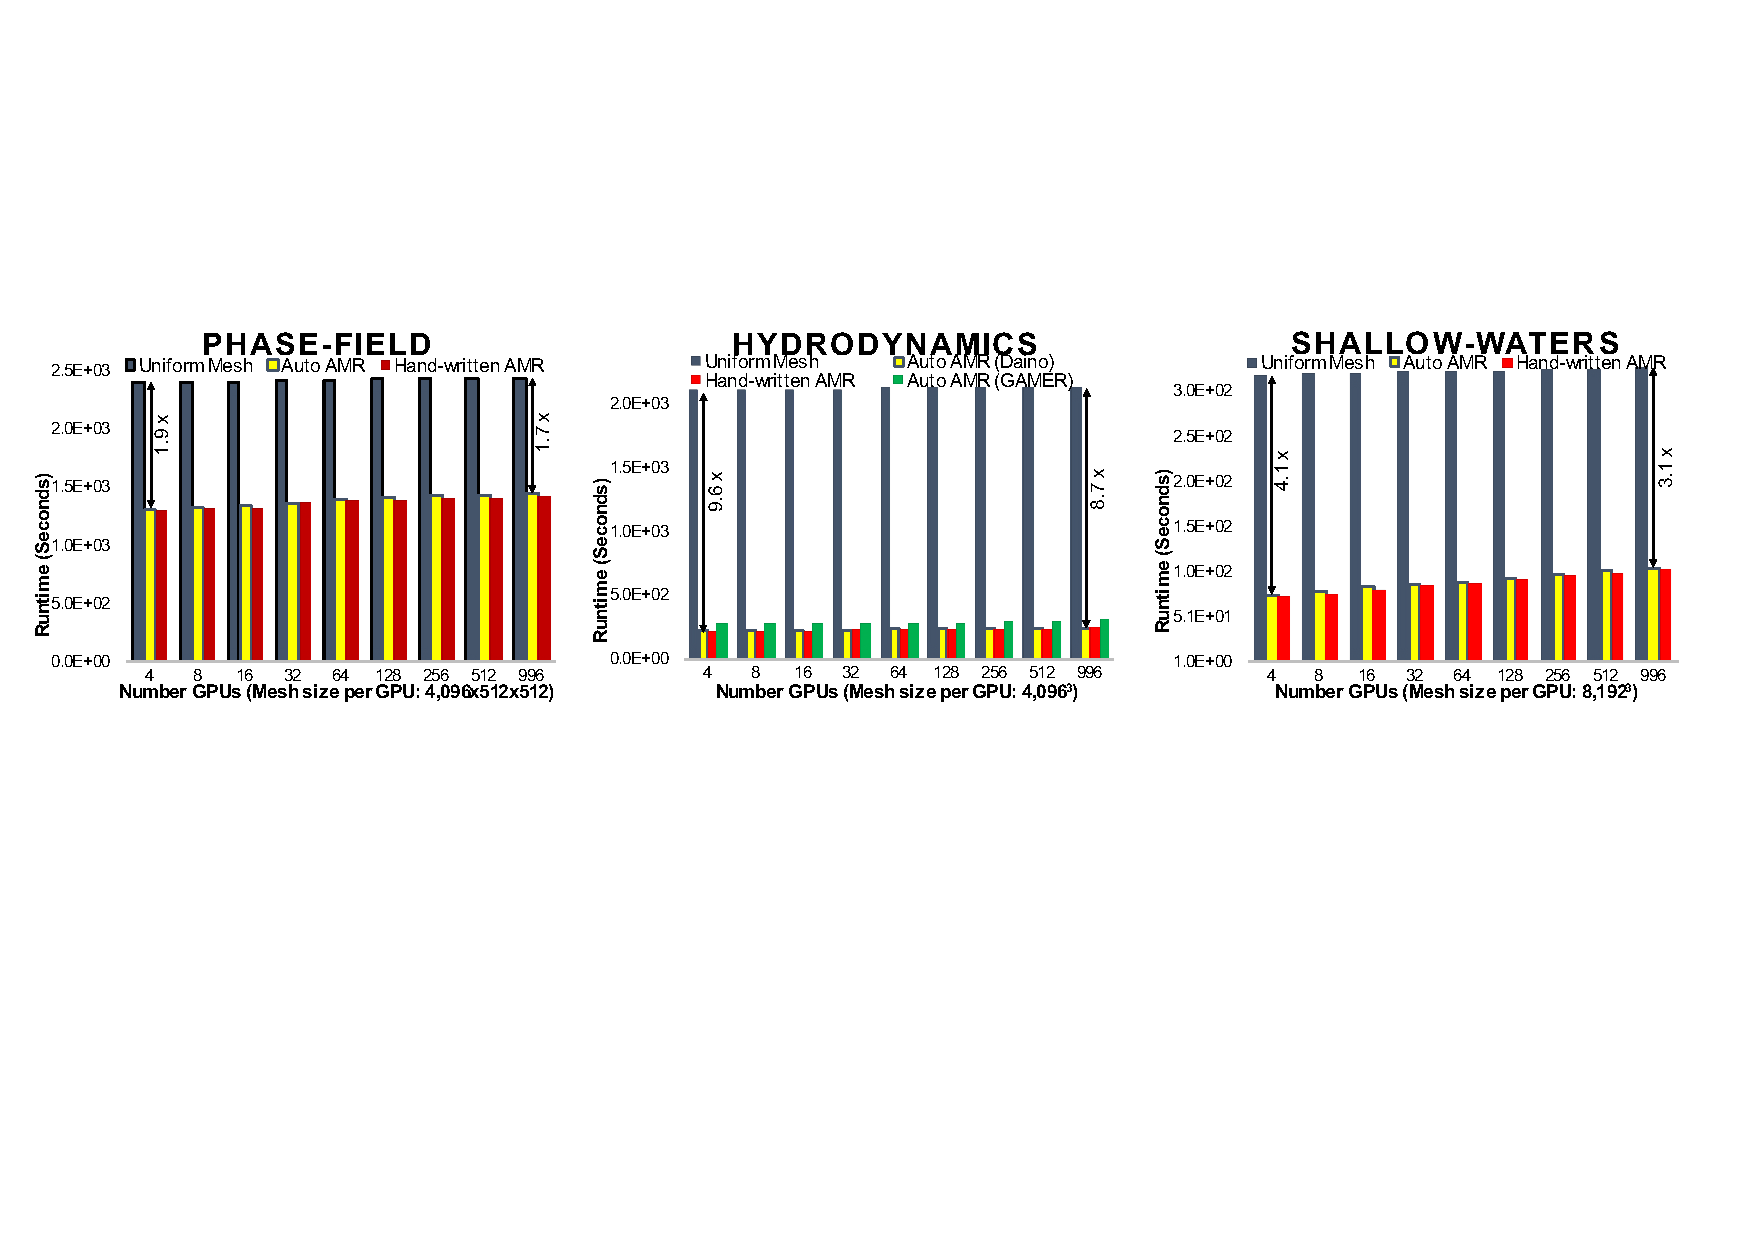
\includegraphics[width=\textwidth]{research/maruyama/wahib01.pdf}%1-expanded.pdf}%1.pdf},
%\caption{Weak scaling of hand-written AMR and Daino-generated AMR versus uniform mesh (Note: GAMER-generated AMR included in hydrodynamic solver)}
\caption{\small{Weak scaling of uniform mesh, hand-written and automated AMR (GAMER-generated AMR included in hydrodynamic)}}
  \locallabel{fig:wahib01}
%%\vspace{-5pt}
\end{figure*}
\begin{figure*}[t]
\centering
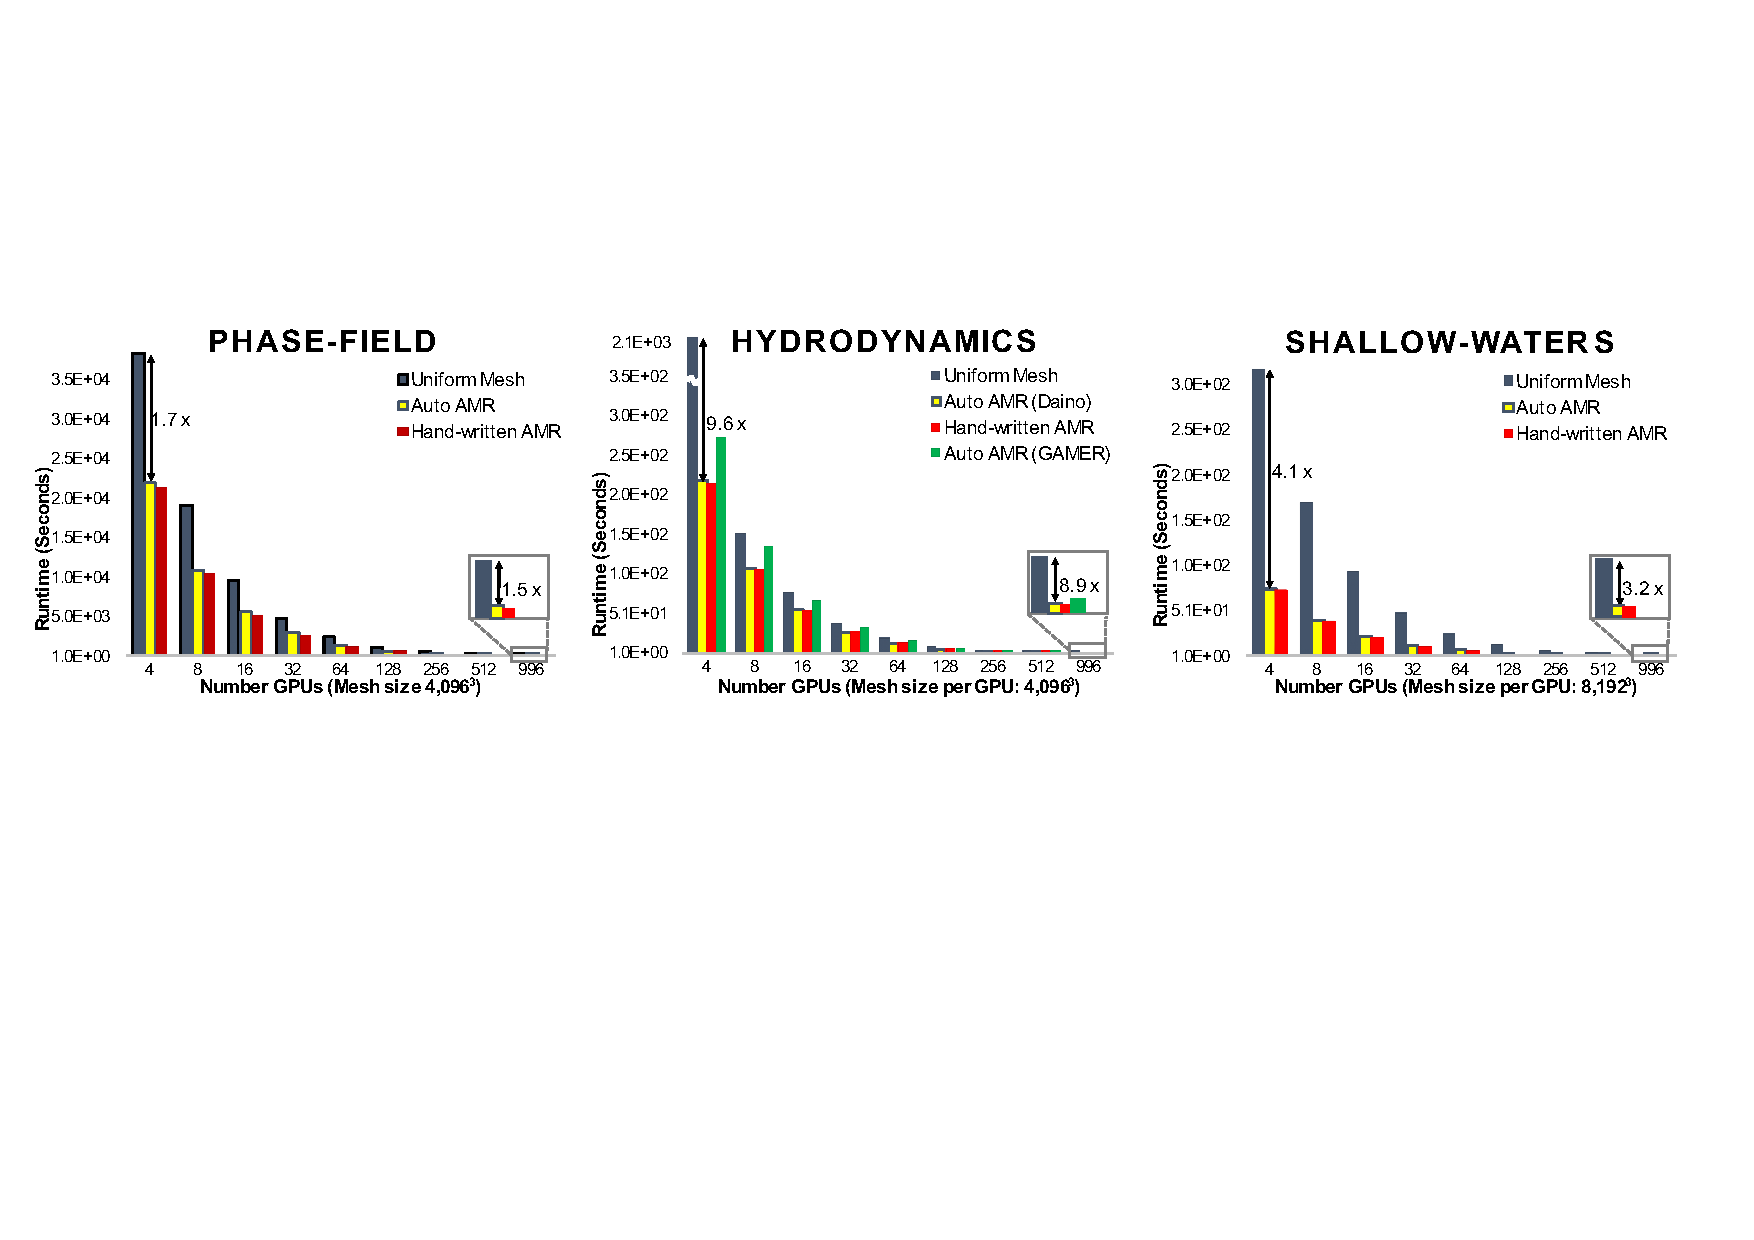
\includegraphics[width=\textwidth]{research/maruyama/wahib02.pdf}%1-expanded.pdf}%1.pdf},
%\caption{Strong scaling of hand-written AMR and Daino-generated AMR versus uniform mesh (Note: GAMER-generated AMR included in hydrodynamic solver)}
\caption{\small{Strong scaling of uniform mesh, hand-written and automated AMR (GAMER-generated AMR included in hydrodynamic)}}
 \locallabel{fig:wahib02}
%%\vspace{-5pt}
\end{figure*}

\textbf{Implementation:}
Our framework consists of a compiler and runtime components. We generate executables optimized for GPU execution by leveraging the LLVM compiler infrastructure. Our compiler builds on the LLVM compiler infrastructure. First, we use the front end to analyze and translate the stencil source code into GPU-optimized code in the form of LLVM Intermediate Representation (IR). Next, compiler passes are applied on the IR to add the AMR management code, which in turn make API calls to: a) the runtime API, and b) the GPU-optimized code generated by Nvidia back end code generator. Finally, LLVM IR is compiled and linked with the runtime libraries to generate an executable. The different stages of the compilation is managed by a shell script that the programmer invokes.

We have built two libraries into the runtime. First, the \emph{AMR library} that encapsulates the AMR hierarchy management software. Second, the \emph{communication library} that wraps the MPI runtime library to simplify data movement operations for the AMR driver.

\textbf{Applications:} We evalute our framework with three production applications. \emph{Phase-field simulation for dendritic growth}: We simulate 3D dendritic growth during solidification in a binary alloy using phase-field model. The computation requires a $2^{nd}$ order finite difference scheme for space with $1^{st}$ forward Euler-type finite difference method for time on a 3D uniform mesh. We use the code by Shimokawabe et. al as our reference implementation. \emph{Hydrodynamics Solver}: We model a hydrodynamics application using 3D Euler equations. We explore a $2^{nd}$ order directionally split hyperbolic schemes to solve the equation. We use the code by GAMER framework for the Hydrodynamics solver as our reference implementation. \emph{Shallow-water Solver}: We model shallow water simulations by depth-averaging the Navier--Stokes equations. We use a numerical method based on a semi-discrete, $2^{nd}$ order, central scheme. To advance the time step, we base our flux, max step, boundary condition, and time integration kernels on the model proposed by Saetra et. al.

\textbf{Experimental Setup:} We use the TSUBAME2.5 supercomputer at Tokyo Tech. Each node has two socket Intel Xeon X5670 2.93GHz CPUs (12 cores), and three Nvidia Kepler K20x GPUs with total 54GB and 18GB of system and GPU memory. The compute nodes are interconnected by dual QDR Infiniband networks with a full bisection-bandwidth fat-tree topology network. We use CUDA v7.0 Toolkit for GPU code and LLVM compiler infrastructure v3.8 for the framework. Single precision variables are adopted in all experiments for all applications. The hand-written and automated AMR versions of all applications use the data-centric AMR approach. All experiments used $16^3$ mesh block size and 2D CUDA thread blocks of size $16$x$16$ threads. All test runs are collected for $100,000$ time steps with a constant maximum of six refinement levels.

\textbf{Results:} In a weak scaling experiment, shown in Figure~\localref{fig:wahib01}, the runtime for uniform mesh, hand-written AMR, and auto-generated AMR are compared. The following points are important to note. First, more than $1.7$x speedup is achieved using our framework with $1000$ GPUs for the phase-field simulation. This is a considerable improvement considering that the uniform mesh implementation is a Gordon Bell prize winner for time-to-solution. Second, we included a comparison with the auto-generated AMR by GAMER framework for the hydrodynamics solver. The AMR code generated by our framework is faster than the code generated by GAMER, mainly because GAMER uses a pipeline to hide data movement latency while our framework uses a data-centric approach to avoid data movement altogether. Third, we achieve good scaling that is comparable to the scalability of the hand-written AMR code.

Figure~\localref{fig:wahib02} shows a strong scaling comparison for hand-written AMR and auto-generated AMR against uniform mesh implementation. The auto-generated AMR by our framework achieves runtime and scalability comparable to that of the uniform mesh implementation. However, when using more GPUs, reduction in speedup starts to occur as the management of AMR starts to dominate the simulation runtime.
\subsection{High Performance Graph Analytics Study with Graph500}
% Maruyama

\section{Schedule and Future Plan}

\subsection{KMR}
% Takizawa & Matsuda

We plan to extend our first research activity (Improve locality when running MPI programs as MapReduce tasks) to improve the representation of programs.
Because the current version depends on key-value pairs as data exchanged between tasks as the usual MapReduce model but supports both serial and parallel MPI execution, we have to distinguish Map functions for these two cases and actually implemented them as different functions.
It is obviously redundant as their objective is the same; mapping data.
Moreover, users can not recognize the number of processes used in each MPI programs run as Map because they are unaware of locations of input key-value pairs and number of processes that hold the input key-value pairs.

To overcome these problems, we are developing a hybrid programming model of MPI message passing and MapReduce model.
In this model, we model data exchanged between tasks as multi-dimensional array which can be split to process each chunk depending on user perspectives at run time.
The location of chunks of the multi-dimensional array is also changeable at run time.
A Map function in this model applies a user-defined function to each chunk of the multi-dimensional array using processes that hold the data.
We are developing the model and applying it to application workflows that perform ensemble simulations.

As for KMRViz, we plan to support more KMR operations to trace and visualize them.

\subsection{High Level Framework for High Performance AMR}
% Wahib
Initially, we intend on testing expanding the framework to allow for user-defined boundary conditions and error estimation functions. We also intend on testing framework at larger scale using TSUBAME2.5 supercomputer (under a grant from JHPCN). Finally, we are closely working with collaborators on FLASH project at Chicago university (Dr. Anshu Dubey) to introduce an integration between our framework and FLASH

\subsection{High Performance Graph Analytics Study with Graph500}
% Maruyama

%%% DO NOT EDIT BELOW

\section{Publications}

%\printbibliography[keyword=journal, heading=subbibliography, title={Journal Articles}, prefixnumbers={1-}, resetnumbers=true]
%\printbibliography[keyword=proceedings, heading=subbibliography, title={Conference Papers}, prefixnumbers={2-}, resetnumbers=true]
%\printbibliography[keyword=invited, heading=subbibliography, title={Invited Talks}, prefixnumbers={3-}, resetnumbers=true]
%\printbibliography[keyword=poster, heading=subbibliography, title={Posters and Presentations}, prefixnumbers={4-}, resetnumbers=true]
%\printbibliography[keyword=deliverable, heading=subbibliography, title={Patents and Deliverables}, prefixnumbers={5-}, resetnumbers=true]

\printbibliography[keyword=journal, heading=subbibliography, title={Journal Articles}, resetnumbers=true]
\printbibliography[keyword=proceedings, heading=subbibliography, title={Conference Papers}]
\printbibliography[keyword=invited, heading=subbibliography, title={Invited Talks}]
\printbibliography[keyword=poster, heading=subbibliography, title={Posters and Presentations}]
\printbibliography[keyword=deliverable, heading=subbibliography, title={Patents and Deliverables}]

\end{refsection}
